\subsubsection{System Boot}
\label{sec:boot}

\begin{figure*}[htb]
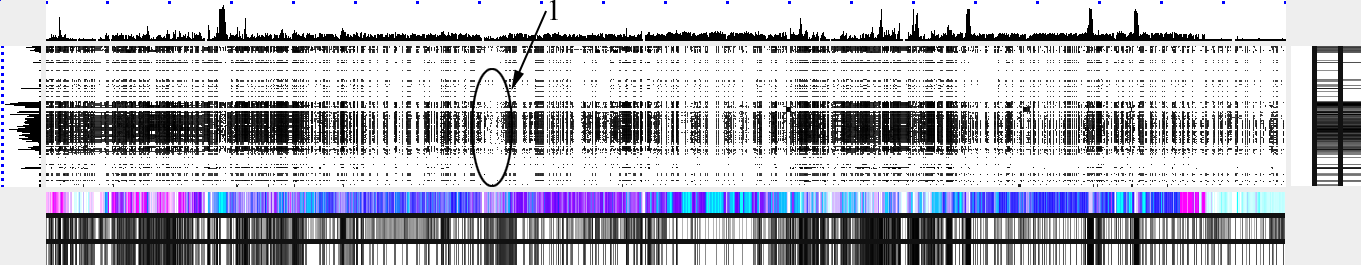
\includegraphics[width=1.0\textwidth]{lviz/boot-dp.png}
\caption{Time-ordered \VDP{} comparing boot
of a clean (Y axis) and a dirty (X axis) system.
}
\label{fig:boot-dp}
%\begin{tabular}{ll}
%DP match : & program + operation + parameter\\
%DP color : & black $\rightarrow$ any\\
%Bar1 color : & cyan $\rightarrow$ Google Desktop; magenta $\rightarrow$ AVG\\
%Bar2 color : & black $\rightarrow$ any program except Google Desktop and AVG\\
%Bar3 color : & black $\rightarrow$ file operation on Windows system directories\\
%\end{tabular}
{\it DP match}: program + operation + parameter;
{\it DP color}: black $\rightarrow$ any;
{\it Bar1 color}: cyan $\rightarrow$ Google Desktop; magenta $\rightarrow$ AVG;
{\it Bar2 color}: black $\rightarrow$ any program except Google Desktop and AVG;
{\it Bar3 color}: black $\rightarrow$ file operation on Windows system directories.
\end{figure*}

In Fig.~\ref{fig:boot-dp}, we use \lviz{} to investigate system boot and try to identify possible
factors causing a system to boot slowly.
To do this, we use a time-ordered \VDP{} to
compare a clean system which is known to boot quickly
with a (dirty) system which has many programs installed and boots slowly.

We see that the clean system boots much faster than the dirty system 
as the height is much shorter than the width.
Whenever Bar2 on the x-axis is not black,
the AVG (AVG antivirus) or Google Desktop is responsible for events.
We see that most of the events in the dirty boot are due to AVG or Google
Desktop.
We can also see from comparing Bar2 with Bar3
that the dirty system has other installed programs running
which are not in Windows directories.
%By looking at Bar1, we can clearly see that Google Desktop and AVG comprise about 5\% of boot time.

Even ignoring other programs outside the Windows directories,
the slowdown is also due to extra work by programs in Windows
directories.
We can see that this because some of the white DP gaps match up with 
black portions in Bar2 (program from Windows directory), e.g. Region 1.
This can be caused by the modification of the Windows system
by third party programs,
e.g. installing new services which are running in svchost.exe, and adding new registry keys or files
which will be scanned by windows programs.
To find out the details, we can focus on Windows built-in programs which
are identified by Bar3.
Vertical gaps in the Windows built-in program region identify the additional work done
by the Windows built-in programs in the dirty system.
By clicking in Region 1, we found out that the gap is caused by
{\tt svchost} (the generic processes for services) since
the new software installed uses {\tt svchost} to run some services.
